
\begin{itemize}
    \item Newton puro, con : $\lambda_k = 1$
\begin{table}[H]
\centering
\renewcommand{\arraystretch}{1.2} 
\begin{tabular}{|c|c|c|c|c|c|c|}
\hline
\textbf{Iter} & \textbf{$x_{inicial}$} &\textbf{$x^k$} & \textbf{||$\nabla \mathbf{f(x^k)}$}|| & \textbf{f($\mathbf{x^k}$)} & \textbf{tiempo} \\
\hline
5  &  (0.09 , 0.43) &( 0.00000,0.00000 ) & 0.00000000 & -1.00000000 & 0.0577 \\
4  &  (0.34 , 0.15) &( -0.00000,-0.00000 ) & 0.00000084 & -1.00000000 & 0.0449 \\\hline
\end{tabular}
\end{table}

\begin{figure}
    \centering
    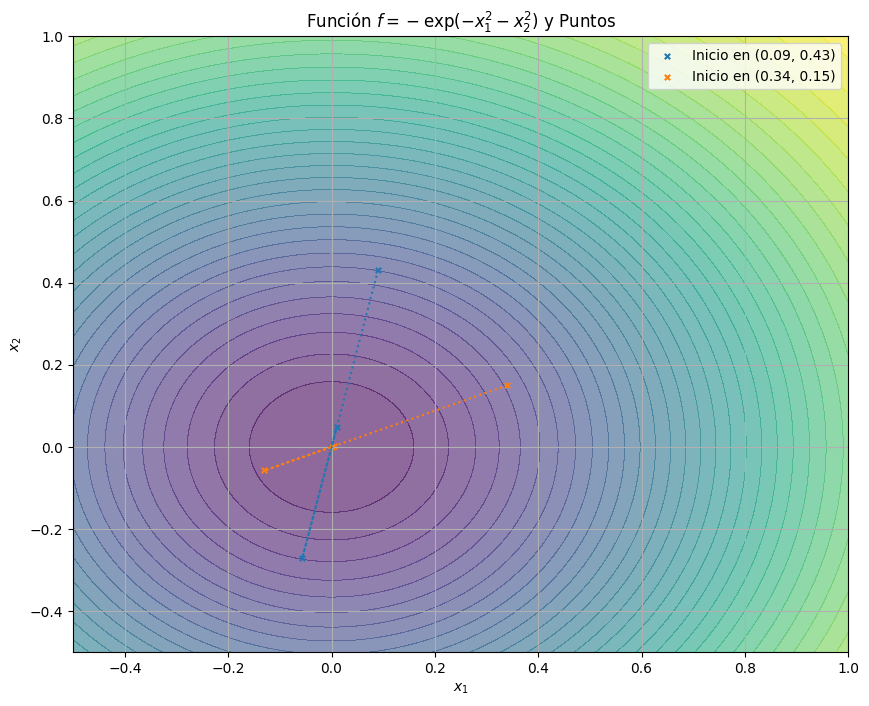
\includegraphics[width=0.65\linewidth]{figuras/PREG5_NEW.png}
    \label{fig:enter-label}
\end{figure}



\begin{itemize}
\item  Hessiana definida no positiva : ( 0.24 ,0.85 )
\item  Hessiana definida no positiva : ( 0.85 ,0.12 )
\item  Hessiana definida no positiva : ( 0.9 ,0.26 )
\item  Hessiana definida no positiva : ( 0.06 ,0.86 )
\item  Hessiana definida no positiva : ( 0.59 ,0.78 )
\item  Hessiana definida no positiva : ( 1.9 ,5.49 )
\item  Hessiana definida no positiva : ( 1.29 ,2.26 )
\item  Hessiana definida no positiva : ( 2.4 ,3.38 )
\item  Hessiana definida no positiva : ( 3.42 ,3.87 )
\item  Hessiana definida no positiva : ( 2.46 ,2.07 )
\item  Hessiana definida no positiva : ( 5.65 ,6.18 )
\item  Hessiana definida no positiva : ( 2.46 ,2.18 )
\item  Hessiana definida no positiva : ( 1.28 ,1.49 )
\item  Hessiana definida no positiva : ( 1.28 ,2.49 )
\item  Hessiana definida no positiva : ( 3.78 ,2.62 )
\end{itemize}









\item Utilizando busqueda exacta.

\begin{table}[H]
\centering
\renewcommand{\arraystretch}{1.2} 
\begin{tabular}{|c|c|c|c|c|c|c|}
\hline
\textbf{Iter} & \textbf{$x_{inicial}$} &\textbf{$x^k$} & \textbf{||$\nabla \mathbf{f(x^k)}$}|| & \textbf{f($\mathbf{x^k}$)} & \textbf{tiempo} \\
\hline
2  &  (0.09 , 0.43) &( 0.00000,0.00000 ) & 0.00000000 & -1.00000000 & 0.2613 \\
2  &  (0.34 , 0.15) &( 0.00000,0.00000 ) & 0.00000000 & -1.00000000 & 0.2652 \\
\hline
\end{tabular}
\end{table}


\begin{figure}
    \centering
    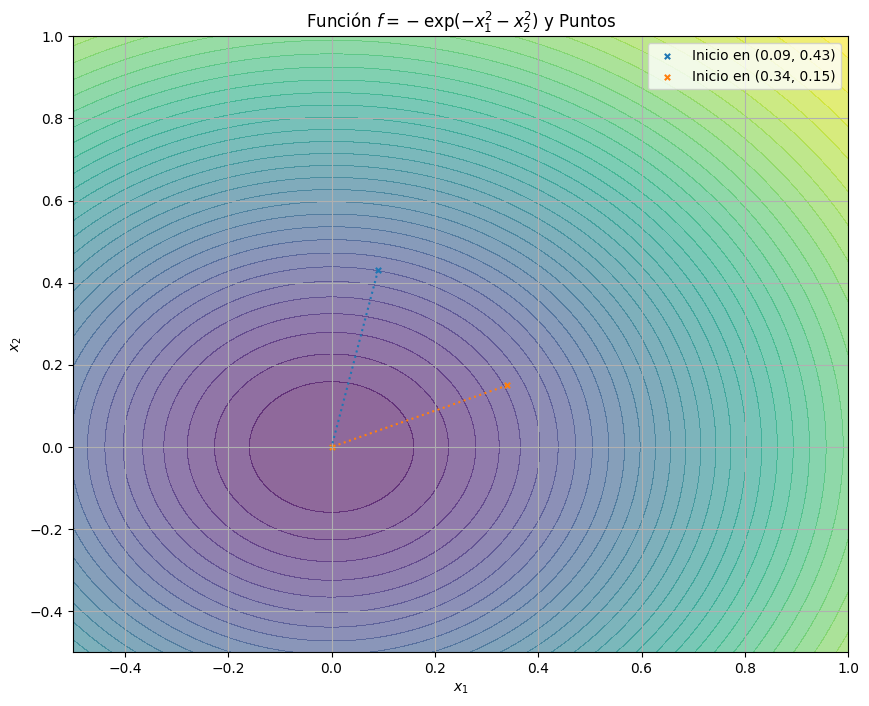
\includegraphics[width=0.65\linewidth]{figuras/PREG5_UNI.png}
    \label{fig:enter-label}
\end{figure}

\item Utilizando busqueda de Armijo


\begin{table}[H]
\centering
\renewcommand{\arraystretch}{1.2}
\begin{tabular}{|c|c|c|c|c|c|c|}
\hline
\textbf{It$_{total}$} & \textbf{Arm$_{total}$} & \textbf{x$_{incial}$} &\textbf{$\mathbf{x^k}$} & \textbf{|| $\nabla$f($\mathbf{x^k}$) ||} & \textbf{f($\mathbf{x^k}$)}&\textbf{tiempo} \\
\hline
14  & 25& (0.09 , 0.43) &( -0.00000,-0.00000 ) & 0.00000000 & -1.00000000 & 0.5776 \\
15  & 27& (0.34 , 0.15) &( -0.00000,-0.00000 ) & 0.00000000 & -1.00000000 & 0.5651 \\
\hline
\end{tabular}
\end{table}
\begin{figure}
    \centering
    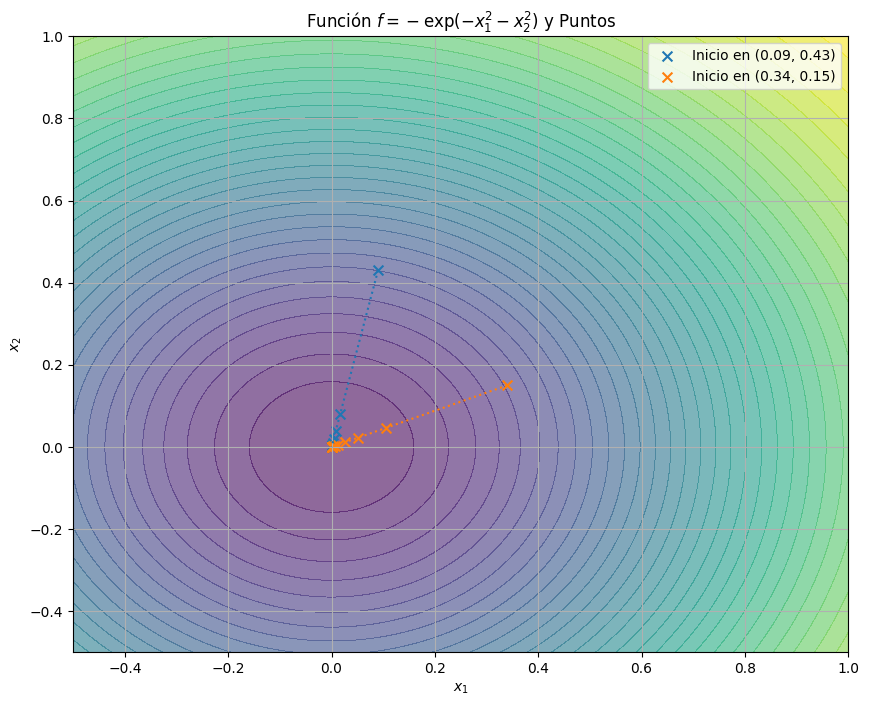
\includegraphics[width=0.65\linewidth]{figuras/PREG5_ARMIJO.png}
    \label{fig:enter-label}
\end{figure}

\end{itemize}




